\appendices
\onecolumn
\section{Prompt operativo de etiquetado por API}
\label{app:prompt_operativo}

El texto siguiente es una transcripción estructurada y completa del archivo \path{03_2_etiquetado_llm_api/prompt_operacional_compacto.md}, versión 1.1. Una copia idéntica reside en \path{03_1_etiquetado_llm/}. El prompt declara que compila la guía, las instrucciones de transporte y la taxonomía; debe revisarse cuando cambie una de ellas.

\subsection*{Rol}

Clasificar chunks de subtítulos de YouTube peruano para priorizar revisión humana, sin actuar como moderador final. Evaluar el efecto del mensaje sobre el blanco aunque el hablante niegue intención o lo presente como humor. La clasificación es multietiqueta e indica todas las categorías aplicables. No usar políticas genéricas de toxicidad, conocimiento previo como taxonomía alternativa ni coincidencias simples de palabras; no inventar etiquetas. Si un modismo o el chunk aislado no se entiende, conservar un daño plausible solo cuando haya evidencia y añadir \texttt{contexto\_necesario}.

\subsection*{Etiquetas permitidas}

\textbf{Seguro.} \texttt{seguro}: información, descripción, narración u opinión sin inferiorización, ataque o amenaza a una persona o grupo. \texttt{seguro\_ironia\_marcada}: ironía o parodia cuyo blanco es una institución, política o situación abstracta y que no daña a un grupo humano. Una etiqueta segura no coexiste con daño ni con la otra etiqueta segura. Una cita dañina solo puede considerarse segura cuando el hablante se opone claramente a ella.

\textbf{Racismo y discriminación.}
\begin{itemize}
\item \texttt{racismo\_etnico\_explicito}: término étnico usado para degradar o inferiorizar, como ``serrano'', ``cholo'', ``negro'', ``indio'', ``chino'', ``cholito'', ``camba'' o ``motoso'' usados como insulto.
\item \texttt{racismo\_linguistico}: burla del acento andino, motoseo, español influido por quechua u ortografía de migrantes o provincianos; esas variedades no son daño por sí mismas.
\item \texttt{clasismo\_racial}: inferiorización por clase con carga étnica, consumo, apariencia o conducta asociada a migrantes o clase baja; incluye, según contexto, ``amixer'', ``huachafa'', ``chusma'', ``cholería'' o ``gente de barrio''.
\item \texttt{discriminacion\_regional}: ataque o inferiorización por ser provinciano, serrano, del interior o de fuera de Lima; incluye centralismo que presenta a Lima como superior.
\item \texttt{racismo\_encubierto}: discriminación étnica o regional presentada como diferencia de educación, cultura, civismo o mérito.
\end{itemize}
Estas etiquetas pueden coexistir. Las fuentes que el prompt nombra para estos criterios son Callirgos, Zavala y Back, Almeida y Zavala, Brañez Medina, Zavala y Zariquiey, y Portocarrero; sus aportes y referencias se desarrollan en la Sec.~II-B.

\textbf{Acoso.}
\begin{itemize}
\item \texttt{misoginia\_acoso\_genero}: ataque por ser mujer, insulto sexualizado, exclusión por género o feminización usada para degradar a un hombre.
\item \texttt{homofobia\_transfobia}: insulto, amenaza, patologización o deslegitimación por orientación sexual o identidad de género.
\item \texttt{acoso\_personal}: ataque dirigido a una persona identificable por nombre, cargo, rol o datos; incluye doxeo, campaña o llamado a terceros. Una crítica política o profesional argumentada no es automáticamente acoso.
\item \texttt{amenaza\_directa}: intención explícita o implícita, pero clara, de daño físico, legal o económico; suele coexistir con acoso personal.
\end{itemize}

\textbf{Contenido sexual.}
\begin{itemize}
\item \texttt{sexual\_explicito}: descripción gráfica de actos sexuales sin necesidad informativa o periodística.
\item \texttt{sexual\_cosificacion}: reducción del valor de una persona a su cuerpo, apariencia o utilidad sexual.
\item \texttt{sexual\_no\_consensual}: material íntimo, grabación, filtración o distribución sin consentimiento.
\end{itemize}

\subsection*{Flags permitidos}

Los flags acompañan un daño, nunca lo reemplazan y siempre activan \texttt{needs\_review=true}. \texttt{ironia\_ambigua} indica que no puede decidirse si el texto critica el daño o lo reproduce con distancia; \texttt{humor\_encubridor}, que el tono jocoso minimiza un daño que permanece al retirar el humor; y \texttt{contexto\_necesario}, que falta antecedente, referente, final de frase, modismo o contexto cultural o audiovisual. Ironía ambigua y contexto necesario limitan la confianza a 0,65. Los tres valores aparecen solo en \texttt{flags}; si no hay daño sustentable, se eliminan y se usa \texttt{labels=["seguro"]}.

\subsection*{Decisión obligatoria en siete pasos}

\begin{enumerate}
\item Identificar el blanco, el hablante o tono y el posible humor, ironía o exageración; el humor no descarta daño.
\item Comprobar si el texto es seguro; una opinión negativa sin inferiorización o ataque puede serlo, y la ironía solo es segura cuando su blanco no es un grupo humano ni produce daño colateral.
\item Revisar por separado los cinco subtipos de racismo y discriminación y asignar todos los aplicables.
\item Revisar misoginia, homofobia o transfobia, ataque a una persona identificable y amenaza.
\item Revisar contenido sexual explícito, cosificación y ausencia de consentimiento, considerando el contexto periodístico.
\item Añadir los flags aplicables; humor e ironía no eliminan un daño sustentado.
\item Verificar que \texttt{labels} no esté vacío; que seguro no coexista con daño; que se hayan incluido todas las etiquetas aplicables; que cualquier flag o score menor que 0,70 active revisión; que ironía o contexto limiten el score a 0,65; y que la justificación sea concreta y breve.
\end{enumerate}

\subsection*{Español peruano y términos sensibles}

\begin{itemize}
\item ``cholo/a'' puede funcionar como identidad, reapropiación o insulto y se decide por contexto; si no es concluyente, se conserva el daño plausible con el flag correspondiente.
\item ``causa'' y ``pata'' suelen ser jerga amistosa, no acoso.
\item ``terruco'' suele ser derogatorio: activa acoso personal si identifica a alguien y puede sumar racismo étnico cuando racializa a una persona o grupo andino.
\item ``amixer'' usado de forma despectiva hacia migrantes andinos activa clasismo racial.
\item ``motoso/a'' como burla activa racismo lingüístico y puede sumar racismo étnico o regional según el blanco.
\item Los canales irónicos requieren revisar el blanco y el género humorístico no concede inmunidad.
\end{itemize}

\subsection*{Salida y ejemplos mínimos}

Para cada fragmento, devolver su identificador, las etiquetas y señales aplicables, la necesidad de revisión, una puntuación de confianza y una justificación breve. Conservar el orden, usar solo el vocabulario permitido y limitar la puntuación al intervalo \([0,1]\). Cualquier señal, puntuación menor que 0,70 o duda justificada activa la revisión. La salida omite texto repetido, metadatos innecesarios y razonamiento interno.

El prompt incluye ocho casos mínimos: una votación como segura; ironía sobre una política como segura marcada; burla al habla andina como racismo lingüístico, étnico y regional con humor encubridor; inferiorización cultural de personas de la sierra como racismo encubierto y regional; mandato de volver a cocinar como misoginia; advertencia de conocer el domicilio como acoso y amenaza; atribución de empleo al cuerpo como cosificación y posible misoginia; y circulación de fotos íntimas como contenido no consensual y posible acoso personal.

\subsection*{Ensamblaje y alcance acreditado}

El proceso antepone la identidad del clasificador, inserta este prompt y la taxonomía completa, y añade reglas para lotes, salida estructurada, orden de identificadores, vocabulario literal y límites de longitud. La llamada usa temperatura 0 y razonamiento desactivado. Los manifiestos de los lotes anotados por API registran la versión del prompt. Este prompt guía la anotación y no forma parte de la entrada textual del clasificador Qwen3--LoRA.


\clearpage
\section{Ejemplos de chunks con puntuaciones altas de Qwen3--LoRA}
\label{app:ejemplos_scores}

\textbf{Advertencia de contenido:} los extractos siguientes reproducen lenguaje discriminatorio, hostil o sexual únicamente para documentar el comportamiento del clasificador; no expresan la posición de los autores. Se seleccionan \emph{post hoc} entre los 5\,324 chunks de validación, sin consultar test. Las puntuaciones proceden del Qwen3--LoRA operacional, en el orden \Rac, \Gen, \Ame{} y \Sex. Los umbrales son 0,225; 0,200; 0,225 y 0,300. Cada ejemplo presenta una sola categoría tanto en la referencia como en la predicción. Los 15 casos priorizan puntuaciones altas y limitan el aporte a un chunk por canal. Se muestran dos cifras significativas; los puntos suspensivos solo acortan el texto.

\subsection*{Valoración segura muy alta}

En el baseline ilustrado, \texttt{SEGURO} se derivaba al no activar ningún daño: se exigieron referencia segura y cuatro scores bajo umbral, y se ordenó por el menor margen \(\min_k(\theta_k-s_k)\). El valor mostrado es \(1-\max_k s_k\), no una probabilidad calibrada por una cabeza segura. Esta construcción no representa la quinta salida aprendida del contrato final.

\begin{enumerate}
\item \textbf{Canal:} \emph{Líbero Deportes}; \(>0,99\): ``Este sábado se juega un partidazo en Matute''.
\item \textbf{Canal:} \emph{Buen Viaje}; \(>0,99\): ``lo que hemos podido aprender de este destino es que [\ldots] tiene unos objetivos en cuidar el medio ambiente''.
\item \textbf{Canal:} \emph{Misias pero viajeras}; \(>0,99\): ``es un centro de exhibición de diferentes tipos de artesanía [\ldots] aproximadamente 150 familias [\ldots] se soportan en base a las donaciones y a las compras''.
\end{enumerate}

\subsection*{Racismo y discriminación}

\begin{enumerate}
\item \textbf{Canal:} \emph{Panamericana Noticias}; 0,96: ``esta es la típica narrativa de que pobrecito el serrano que no piensa, que no sabe nada [\ldots] me molesta esta superioridad''.
\item \textbf{Canal:} \emph{Juanito y Richard}; 0,95: ``ese indio no [\ldots] habla''.
\item \textbf{Canal:} \emph{ATV Noticias}; 0,83: ``Es los venezolanos [\ldots] ellos son los que hacen''.
\end{enumerate}

\subsection*{Ataque por género e identidad}

\begin{enumerate}
\item \textbf{Canal:} \emph{Todo Good}; 0,81: ``eso no te hace ser una chica [\ldots] no me sentiría cómoda ni segura que en el baño de niñas entren hombres [\ldots] que [\ldots] se perciban chicas''.
\item \textbf{Canal:} \emph{Sin Guion con Rosa Maria Palacios}; 0,68: ``O tienes mucho enclosetado ahí adentro [\ldots] están todos son gays, menos yo''.
\item \textbf{Canal:} \emph{Magaly TV La Firme}; 0,45: ``tiene el vicio de sacar la vuelta y estar con diferentes hombres''.
\end{enumerate}

\subsection*{Acoso y amenaza}

\begin{enumerate}
\item \textbf{Canal:} \emph{Arde Troya con Juliana Oxenford}; 0,90: ``Pienso que es un cobarde [\ldots] hoy eres un cobarde''.
\item \textbf{Canal:} \emph{Perú Actual}; 0,87: ``te voy a matar''.
\item \textbf{Canal:} \emph{Nunca MAS}; 0,87: ``yo te encuentro con alguien yo te mato [\ldots] pero ya estás muerta''.
\end{enumerate}

\subsection*{Contenido sexual}

\begin{enumerate}
\item \textbf{Canal:} \emph{Hablando Huevadas}; 0,94: ``cuando duermo con ella [\ldots] tengo la mano en su poto''.
\item \textbf{Canal:} \emph{Goblinciano}; 0,38: ``compartieron un audio [\ldots] en pleno polvo [\ldots] pedía a una flaca que diga su nombre mientras cachaban''.
\item \textbf{Canal:} \emph{Nada Espacial}; 0,37: ``empezó a pasar calato [\ldots] por toda la pichula''.
\end{enumerate}

Estos ejemplos ilustran señales que el modelo ordenó por encima de los umbrales. Score alto significa salida calibrada alta respecto del corte, no certeza humana ni probabilidad literal de que la referencia sea correcta. Las referencias provienen de supervisión asistida; los ejemplos no estiman desempeño por subtipo, no sustituyen las métricas sobre test y no autorizan decisiones automáticas sobre personas o videos.


\clearpage
\begin{landscape}
\section{Interfaces de anotación y operación}
\label{app:interfaces}

La Fig.~\ref{fig:interfaz_etiquetado} muestra la versión final del entorno de revisión humana con un chunk real del corpus. La propuesta de DeepSeek Pro aparece antes de decidir y deja tres acciones explícitas: aceptarla, rechazar el caso o modificar las categorías y señales antes de guardar la versión humana. El contador corresponde a la campaña integrada que alimenta esta interfaz.

\begin{figure}[H]
\centering
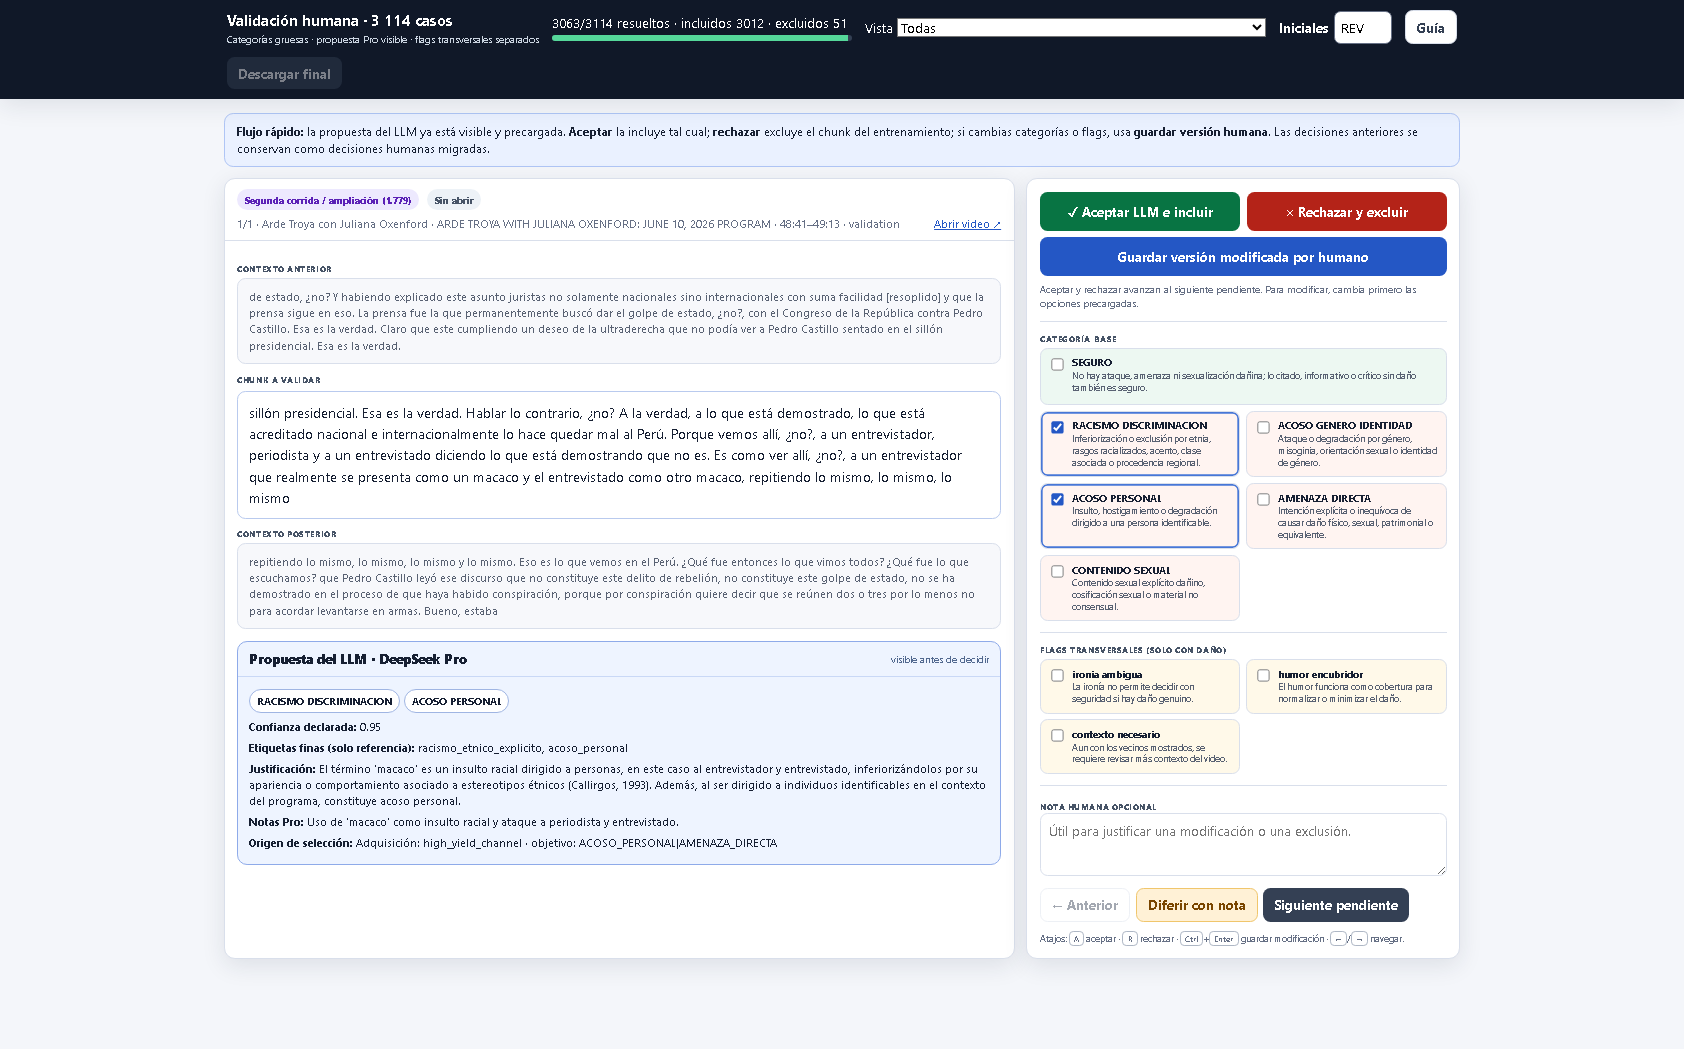
\includegraphics[width=.98\linewidth,height=.78\textheight,keepaspectratio]{figuras/captura_entorno_etiquetado.png}
\caption{Entorno final de revisión humana: texto y contexto, propuesta visible del LLM y controles para aceptar, rechazar o modificar. Captura local del artefacto del proyecto con un registro real.}
\label{fig:interfaz_etiquetado}
\end{figure}

\clearpage

La Fig.~\ref{fig:interfaz_operacion} presenta el demostrador después de enviar por su formulario un chunk real de validación al servidor del paquete desplegable. Qwen3--LoRA asigna 0,94 a contenido sexual; la política operativa conserva el caso como alerta de confianza baja y solicita revisión por su cercanía al umbral. La pantalla muestra la entrada enviada, la respuesta del servidor, los puntajes por categoría y los controles humanos. Cuando la entrada es un video de YouTube, la misma interfaz añade el reproductor y los enlaces temporales a los fragmentos señalados.

\begin{figure}[H]
\centering
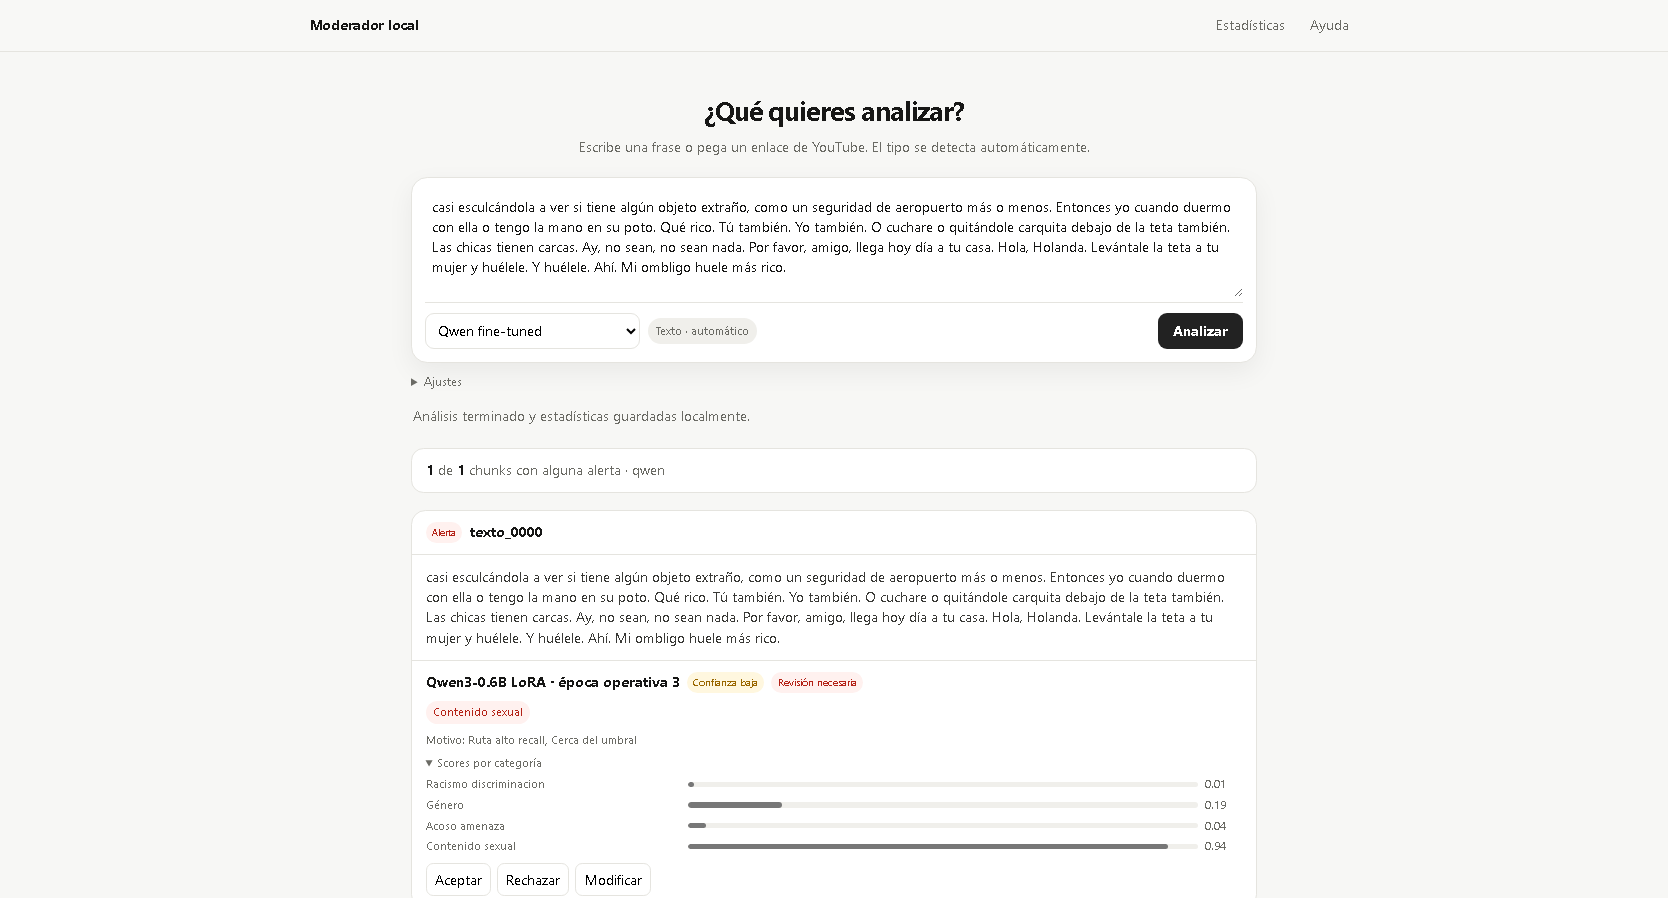
\includegraphics[width=.98\linewidth,height=.78\textheight,keepaspectratio]{figuras/captura_entorno_operacion.png}
\caption{Ejecución real del servidor del paquete desplegable: el formulario envía un chunk de validación, registra una inferencia nueva y muestra la alerta, los puntajes de Qwen3--LoRA y las acciones de revisión humana.}
\label{fig:interfaz_operacion}
\end{figure}

\end{landscape}

\clearpage
\begin{landscape}
\section{Ontología de conceptos y trazabilidad}
\label{app:ontologia}

La Fig.~\ref{fig:ontologia} presenta la ontología del proyecto. Su función es semántica y de trazabilidad: cada predicción refiere a una categoría y a un chunk de evidencia; una decisión humana es un evento posterior, no otra palabra para predicción. El archivo \texttt{ontologia\_moderacion.ttl} expresa clases y propiedades en OWL~2, sintaxis RDF/Turtle y definiciones SKOS \cite{w3c2012owl2,w3c2014turtle,w3c2009skos}.

\begin{figure}[H]
\centering
\resizebox{0.99\linewidth}{!}{\begin{tikzpicture}[
  x=1cm,y=1cm,
  font=\small,
  class/.style={draw,rounded corners=2pt,text width=34mm,minimum height=13mm,align=center,fill=blue!7,inner sep=3pt},
  label/.style={class,fill=orange!11},
  process/.style={class,fill=green!10},
  artifact/.style={class,fill=purple!8},
  relation/.style={-{Stealth[length=2mm]},thick},
  isa/.style={relation,dashed},
  edgeword/.style={font=\footnotesize,fill=white,inner sep=1.5pt},
  lane/.style={font=\small\bfseries,text=black!70,anchor=west}
]
% La mayor separación vertical y la tipografía ampliada priorizan la lectura
% al ancho de una página A4 de una columna.
\node[lane] at (-1.75,1.05) {Evidencia y etiquetado};
\node[class] (video) at (0,0) {Video público};
\node[class] (subtitle) at (6,0) {Pista de subtítulos};
\node[class] (chunk) at (12,0) {Chunk de evidencia};
\node[label] (labeling) at (18,0) {Etiquetado};
\draw[relation] (video.east)--node[edgeword,above]{contiene}(subtitle.west);
\draw[relation] (subtitle.east)--node[edgeword,above]{segmenta}(chunk.west);
\draw[relation] (chunk.east)--node[edgeword,above]{etiqueta}(labeling.west);

\node[artifact] (dataset) at (12,-2.9) {Artefacto de datos\\versión y partición};
\node[label] (concept) at (18,-2.9) {Concepto de\\moderación};
\draw[relation] (chunk.south)--node[edgeword,right]{integra}(dataset.north);
\draw[relation] (labeling.south)--node[edgeword,right]{clasifica}(concept.north);

\node[lane] at (-1.75,-4.7) {Taxonomía operativa};
\node[label] (safe) at (6,-6.0) {Estado \texttt{SEGURO}\\derivado};
\node[label] (damage) at (12,-6.0) {Categoría operativa\\multietiqueta};
\node[label] (fine) at (18,-6.0) {Fenómeno fino\\o señal de revisión};
\coordinate (conceptdrop) at (18,-4.4);
\coordinate (conceptbus) at (15,-4.4);
\draw[dashed,thick] (concept.south) -- (conceptdrop) -- (conceptbus);
\fill (conceptbus) circle (1.1pt);
\draw[isa] (conceptbus) -| (damage.north);
\draw[isa] (conceptbus) -| (fine.north);
\draw[relation] (damage.west)--node[edgeword,above,align=center]{si ninguna\\se activa}(safe.east);

\node[lane] at (-1.75,-8.2) {Inferencia, decisión y retroalimentación};
\node[process] (model) at (0,-9.6) {Modelo versionado};
\node[process] (prediction) at (6,-9.6) {Predicción\\score y umbral};
\node[process] (review) at (12,-9.6) {Decisión humana\\aceptar, modificar\\o rechazar};
\node[artifact] (feedback) at (18,-9.6) {Registro reentrenable\\decisiones versionadas};
\draw[relation] (model.east)--node[edgeword,above]{produce}(prediction.west);
\draw[relation] (prediction.east)--node[edgeword,above,align=center]{si requiere\\revisión}(review.west);
\draw[relation] (review.east)--node[edgeword,above]{registra}(feedback.west);

% Carril izquierdo: solo los datos de entrenamiento alimentan el modelo.
\coordinate (trainlane) at (-2.35,-2.9);
\draw[relation] (dataset.west) -- (trainlane) |- (model.west);
\node[edgeword,anchor=east] at (-2.35,-7.35) {entrena};

% Carril central: la predicción refiere a una categoría sin atravesar nodos.
\coordinate (predictlane) at (9,-7.65);
\draw[relation] (prediction.north) -- (prediction.north |- predictlane) -| (damage.south);
\node[edgeword] at (9,-7.65) {predice};

% La retroalimentación crea una versión futura; no modifica el corpus evaluado.
\coordinate (futurelane) at (18,-11.35);
\draw[isa] (feedback.south) -- (futurelane) -| (model.south);
\node[edgeword,below] at (9,-11.35) {futura iteración DSR};
\end{tikzpicture}
}
\caption{Grafo ontológico de trazabilidad. Línea continua: relación de proceso; discontinua: especialización o retorno a una iteración futura. Elaboración propia con base conceptual en \cite{gruber1993ontology,w3c2012owl2}.}
\label{fig:ontologia}
\end{figure}

\clearpage
La Tabla~\ref{tab:ontologia} fija la definición operacional y la regla de trazabilidad de cada término usado en el grafo.

\begin{table}[H]
\centering
\caption{Vocabulario controlado y regla de uso en el artículo}
\label{tab:ontologia}
\normalsize
\renewcommand{\arraystretch}{1.16}
\begin{tabularx}{\linewidth}{>{\bfseries\raggedright\arraybackslash}p{40mm}X X}
\toprule
\textbf{Término} & \textbf{Definición operacional} & \textbf{Regla de trazabilidad / fundamento} \\
\midrule
Video público & Recurso de YouTube aceptado por los criterios de adquisición. & Conserva \texttt{video\_id}; no implica muestra representativa. \\
Pista de subtítulos & Texto manual o automático con tiempos, disponible para el video. & No se denomina transcripción de audio propia; el proyecto no usó ASR. \\
Chunk & Unidad textual cerrada al alcanzar 30 s o 600 caracteres, con mínimo 90; antes se depura repetición VTT de hasta 12 palabras. & Toda alerta debe enlazar \texttt{chunk\_id}, video e intervalo. No existe solapamiento intencional entre chunks. \\
Anotación & Asignación versionada de conceptos a un chunk. & Distinguir Flash, Pro y revisión final asistida; documentar población y procedencia \cite{bender2018datastatements}. \\
Daño operativo & Una o más de cuatro categorías activables. & Es multietiqueta \cite{tsoumakas2007multilabel}; no equivale a infracción legal. \\
Fenómeno fino / flag & Subtipo descriptivo o indicador transversal de ambigüedad. & Un flag no es daño; gold fino no entra como predictor. \\
SEGURO & Estado derivado si ningún daño supera su umbral. & No es una quinta etiqueta independiente ni prueba de ausencia real de daño. \\
Score / umbral & Salida continua y corte fijado en validación. & No llamar probabilidad sin calibración \cite{niculescu2005probabilities}. \\
\(\AP\) & \(\sum_n(R_n-R_{n-1})P_n\), macro entre daños. & Precisión promedio no interpolada; los archivos dicen PR-AUC \cite{sklearn2026averageprecision}. \\
Alerta / revisión & Enrutamiento selectivo de una predicción incierta o dañina. & No es sanción; el supervisor acepta, rechaza o modifica \cite{chow1970reject,geifman2017selective,andersen2021rem,mozannar2020defer}. \\
Operación semiautomática & Servicio que prioriza, presenta evidencia y registra la decisión del supervisor. & Es el alcance implementado por el frontend; afectar usuarios exige validación prospectiva y gobierno operativo. \\
Artefacto DSR & Conjunto de corpus, modelos, reglas, interfaz, registros y documentación. & Se construye y evalúa iterativamente \cite{hevner2004dsr,peffers2007dsrm}. \\
\bottomrule
\end{tabularx}
\end{table}
\end{landscape}

\clearpage
\section{Detalle de fuentes del corpus}
\label{app:fuentes_dataset}

La Tabla~\ref{tab:categoriasfuente} desagrega el tipo de contenido registrado en los metadatos del corpus integrado. “Muestreo dirigido” describe un régimen de adquisición y no un género editorial; por ello no debe interpretarse como prevalencia de YouTube. La identidad se reconstruye mediante el \texttt{channel\_id} y las URL preservadas en los metadatos de adquisición. Después de unificar aliases y variantes de escritura, los 3\,230 videos proceden de 250 canales únicos.

\begin{table}[H]
\centering
\caption{Chunks y daños por categoría de fuente}
\label{tab:categoriasfuente}
\small
\renewcommand{\arraystretch}{1.08}
\begin{tabular*}{\textwidth}{@{\extracolsep{\fill}}lrrrrrrr@{}}
\toprule
\textbf{Categoría de fuente} & \textbf{Chunks} & \textbf{Videos} & \textbf{Algún daño} & \Rac & \Gen & \Ame & \Sex \\
\midrule
Muestreo dirigido & 47\,395 & 1\,374 & 3\,450 & 793 & 948 & 1\,687 & 1\,325 \\
Humor streaming & 11\,812 & 72 & 1\,621 & 395 & 688 & 232 & 758 \\
Política actualidad & 9\,212 & 449 & 102 & 32 & 8 & 69 & 0 \\
Política análisis & 7\,858 & 150 & 233 & 32 & 21 & 193 & 3 \\
Política periodismo & 7\,583 & 150 & 89 & 13 & 13 & 68 & 0 \\
Humor podcast & 6\,223 & 69 & 108 & 22 & 39 & 20 & 39 \\
Política opinión & 5\,895 & 173 & 282 & 59 & 42 & 194 & 21 \\
Streaming opinión & 5\,155 & 148 & 879 & 378 & 128 & 462 & 76 \\
Viajes & 4\,877 & 149 & 3 & 2 & 0 & 0 & 1 \\
Viajes gastronomía & 4\,404 & 150 & 10 & 3 & 3 & 2 & 3 \\
Deportes informal & 1\,867 & 66 & 4 & 2 & 1 & 1 & 0 \\
Humor comedia & 1\,673 & 74 & 158 & 98 & 44 & 39 & 22 \\
Farándula digital & 1\,478 & 44 & 32 & 5 & 4 & 12 & 12 \\
Farándula & 1\,092 & 75 & 88 & 21 & 20 & 48 & 22 \\
Deportes & 448 & 74 & 4 & 1 & 2 & 1 & 0 \\
Gastronomía & 272 & 13 & 0 & 0 & 0 & 0 & 0 \\
\bottomrule
\end{tabular*}
\end{table}

La Tabla~\ref{tab:fuenteetiqueta} separa la fuente de adquisición de la procedencia de supervisión. Los casos con daño, baja confianza o discrepancias pasan a DeepSeek Pro o a revisión humana asistida.

\begin{table}[H]
\centering
\caption{Procedencia de las etiquetas del corpus integrado}
\label{tab:fuenteetiqueta}
\small
\begin{tabular}{lrrrrrr}
\toprule
\textbf{Fuente de etiqueta} & \textbf{Chunks} & \textbf{Seguro} & \textbf{Daño} & \textbf{Incidencias} & \textbf{Multidaño} & \textbf{Peso base} \\
\midrule
Flash pseudoetiqueta & 93\,636 & 93\,636 & 0 & 0 & 0 & \(0,50\times\) confianza \\
Pro y minería Pro & 20\,516 & 15\,959 & 4\,557 & 5\,426 & 834 & 1 \\
Revisión final asistida & 3\,092 & 586 & 2\,506 & 3\,701 & 961 & 1 \\
\midrule
\textbf{Total} & \textbf{117\,244} & \textbf{110\,181} & \textbf{7\,063} & \textbf{9\,127} & \textbf{1\,795} & \\
\bottomrule
\end{tabular}
\end{table}

Las filas de revisión humana final conservan la decisión y su procedencia para mantener la trazabilidad del corpus.

\subsection*{Canales incluidos y direcciones web}

El inventario se limita a los videos presentes en el corpus integrado. La Tabla~\ref{tab:canales_dataset} presenta por separado los canales con más de dos videos y reúne los canales con uno o dos en una fila final denominada ``Otros''. El conteo permite comprobar la concentración por canal; las direcciones individuales de los canales agrupados permanecen en los metadatos del corpus.

\begingroup
\footnotesize
\setlength{\LTpre}{4pt}
\setlength{\LTpost}{4pt}
% No editar manualmente: regenerar después de cambiar el corpus final.
\begin{longtable}{>{\raggedright\arraybackslash}p{50mm}>{\raggedright\arraybackslash}p{103mm}r}
\caption{Canales con más de dos videos en el corpus final y agrupación de canales con uno o dos}\label{tab:canales_dataset}\\
\toprule
\textbf{Canal} & \textbf{Dirección web principal} & \textbf{Videos} \\
\midrule
\endfirsthead
\multicolumn{3}{c}{\tablename\ \thetable\ (continuación)} \\
\toprule
\textbf{Canal} & \textbf{Dirección web principal} & \textbf{Videos} \\
\midrule
\endhead
\midrule
\multicolumn{3}{r}{Continúa en la página siguiente} \\
\endfoot
\bottomrule
\endlastfoot
24 Horas & \url{https://www.youtube.com/channel/UCsakKsRww3J7pM6DavkrAIQ} & 18 \\
A24com & \url{https://www.youtube.com/channel/UCR9120YBAqMfntqgRTKmkjQ} & 3 \\
AGENCIA EFE & \url{https://www.youtube.com/channel/UCvJS-YNyaWyOucx8bGrHVvw} & 3 \\
América Noticias & \url{https://www.youtube.com/channel/UCPhm2I2wk4vqjENwhn3px8A} & 18 \\
América Televisión & \url{https://www.youtube.com/channel/UCGGry4kGWZUqIfG6LLNhOmg} & 8 \\
Arde Troya con Juliana Oxenford & \url{https://www.youtube.com/channel/UCgEabnv1xth8-qeWqMsTmDw} & 185 \\
ATV Noticias & \url{https://www.youtube.com/channel/UCYG5uXS3xdsoaXIxum1pAEw} & 137 \\
Buen Viaje & \url{https://www.youtube.com/channel/UCpTyTnL_1Hs6LyfD4L2rkpw} & 74 \\
Buenos Días Perú & \url{https://www.youtube.com/channel/UCFnOwPrJ-Skrzk_GPNBV5tg} & 70 \\
Caso Cerrado & \url{https://www.youtube.com/channel/UCGbofRROopWrumVob5w61OA} & 3 \\
Chimi chimi & \url{https://www.youtube.com/channel/UCt42aXXEokQWROe3CdVx3bA} & 4 \\
Ciudadaniasx & \url{https://www.youtube.com/channel/UCt78tVTNhK4hd9l0Io3vTtg} & 3 \\
Cocina Cajamarquina & \url{https://www.youtube.com/channel/UC2lyekNE9NOGWu1R0L8046A} & 13 \\
Cosmos Televisión & \url{https://www.youtube.com/channel/UC_ept7M1UXlCfvcUrK49Ziw} & 10 \\
CTV Perú Oficial & \url{https://www.youtube.com/channel/UCy4UKhdd5U0cUru_sBn-DGA} & 3 \\
DÍA D & \url{https://www.youtube.com/channel/UCmrzeYkbupPuvrXH8roR__w} & 8 \\
Diario El Popular & \url{https://www.youtube.com/channel/UCC25ArAc6QI7yj1UQG8lqxA} & 4 \\
El Búho pe & \url{https://www.youtube.com/channel/UC6xAnp5ygm8oNoBDCgu70UQ} & 3 \\
El diario de Curwen & \url{https://www.youtube.com/channel/UCHUD6A_lv3OXbzgVXwomtkw} & 73 \\
El Dominical de Panamericana & \url{https://www.youtube.com/channel/UCMfcN0OV7d61cWPLYm5qHpw} & 8 \\
El Universal & \url{https://www.youtube.com/channel/UC2SEk1w7DgoHs_G3w1biz-w} & 6 \\
enlacenacional & \url{https://www.youtube.com/channel/UC_Zpz_cv69p4oL0hDEJz4IA} & 6 \\
EXCELSIOR & \url{https://www.youtube.com/channel/UClqo4ZAAZ01HQdCTlovCgkA} & 3 \\
Exitosa Noticias & \url{https://www.youtube.com/channel/UCxgO_rak_BKZP8VNVmYqbWg} & 97 \\
Farandula Politica & \url{https://www.youtube.com/channel/UCEPKBntK_q0AXblXJtDUNhg} & 3 \\
Goblinciano & \url{https://www.youtube.com/channel/UCO0cdOFdG-3hxa_VPG8imnw} & 236 \\
Hablando Huevadas & \url{https://www.youtube.com/channel/UCba1vMvOHWlMddLARS382Zw} & 182 \\
Instarandula & \url{https://www.youtube.com/channel/UC2EkQJU0Ani3SLAVS07MBJg} & 42 \\
Juanito y Richard & \url{https://www.youtube.com/channel/UCfiBnBtw8iNbX8vL4f6cp0Q} & 181 \\
L1MAX & \url{https://www.youtube.com/channel/UCGVHVLD7Nzw0zdIwbVhE3vw} & 66 \\
La República - LR+ & \url{https://www.youtube.com/channel/UC-B7Xv56uNRDkj0vC3QW8Cg} & 16 \\
Latina Noticias & \url{https://www.youtube.com/channel/UCpSJ5fGhmAME9Kx2D3ZvN3Q} & 193 \\
Latina Televisión & \url{https://www.youtube.com/channel/UC3rDtLrcgr3JS3_3JOW4BAw} & 11 \\
Líbero Deportes & \url{https://www.youtube.com/channel/UCk2OZrA0E6q6xp4bBKtf9KA} & 74 \\
LP - Pasión por el Derecho & \url{https://www.youtube.com/channel/UCDscRlCxFfuHhsJBlVvPBmA} & 12 \\
Magaly TV La Firme & \url{https://www.youtube.com/channel/UCF6s3gpbZEQKqZ38VvQ0gLA} & 162 \\
Marco Sifuentes / Ocram & \url{https://www.youtube.com/channel/UCP0AJJeNkFBYzegTTVbKhPg} & 75 \\
Misias pero viajeras & \url{https://www.youtube.com/channel/UCknQM__AyaqSdxunkqpavDg} & 75 \\
Nada Espacial & \url{https://www.youtube.com/channel/UCfwkQ4lY6UO-6K_REQ8CnNQ} & 69 \\
Noticias Caracol & \url{https://www.youtube.com/channel/UC2Xq2PK-got3Rtz9ZJ32hLQ} & 3 \\
Nunca MAS & \url{https://www.youtube.com/channel/UCFqwxsa2Wp6Y5FkUAcGShGA} & 13 \\
Panamericana Noticias & \url{https://www.youtube.com/channel/UCOyD-kV3zB8Cm4LI4qtd9tA} & 75 \\
Panamericana Televisión & \url{https://www.youtube.com/channel/UCngb4rxO4iUE6BrIs29WXwA} & 6 \\
Panorama & \url{https://www.youtube.com/channel/UCBiq92lt_ufNO-ktZigVXgg} & 92 \\
QUE HAY DE NUEVO PERU & \url{https://www.youtube.com/channel/UCRl1-oM_NM-BtCEyTFd-aRA} & 5 \\
RPP Noticias & \url{https://www.youtube.com/channel/UC5j8-2FT0ZMMBkmK72R4aeA} & 122 \\
Sin Guion con Rosa Maria Palacios & \url{https://www.youtube.com/channel/UCdyaE7KCDAD3NYl9r9C69-g} & 75 \\
SOL TV Perú & \url{https://www.youtube.com/channel/UCT3jhkKbEV4ZslnzhZ26hPw} & 3 \\
Tío Lenguado y Descocaos & \url{https://www.youtube.com/channel/UCvPVK5xvxJRY1obR9XRrMfw} & 75 \\
Todo Good & \url{https://www.youtube.com/channel/UC-f4h9oSW5JreShkauu0m1A} & 148 \\
TVPerú Noticias & \url{https://www.youtube.com/channel/UCkZCoc42IipR1ucqJmIehsA} & 54 \\
Viaja y Prueba & \url{https://www.youtube.com/channel/UCD8fpCkckYmYj_qm6hhE4jw} & 75 \\
Wayka & \url{https://www.youtube.com/channel/UCQmo59tWId4OHTdl4W320DQ} & 7 \\
Willax Television & \url{https://www.youtube.com/channel/UCort3mldTtMErPqprSlSfng} & 102 \\
\midrule
Otros (196 canales con uno o dos videos) & Direcciones canónicas conservadas en los metadatos del corpus & 218 \\
\end{longtable}

\endgroup

\clearpage
\section{Disponibilidad y reutilización}
\label{app:disponibilidad}

La Tabla~\ref{tab:repositorios} separa las dos ubicaciones del proyecto. GitHub ofrece el código y el historial de cambios; Drive preserva los bytes empleados por los experimentos y los pesos que no se versionan en Git. El acceso a Drive requiere autorización del equipo.

\begin{table}[H]
\centering
\caption{Ubicación, contenido y condiciones de acceso de los artefactos}
\label{tab:repositorios}
\footnotesize
\begin{tabularx}{\textwidth}{p{18mm}>{\raggedright\arraybackslash}p{82mm}>{\raggedright\arraybackslash}X p{25mm}}
\toprule
\textbf{Sitio} & \textbf{Enlace} & \textbf{Contenido y formatos} & \textbf{Acceso} \\
\midrule
GitHub & \url{https://github.com/lkoc/Trabajo_PLN-MIA-Grupo4} & Scripts Python, cuadernos IPYNB, documentación y archivos de datos versionables. & Público; sin licencia explícita de reutilización \\
Google Drive & \url{https://drive.google.com/drive/folders/1H3PKr7CWd-RwavZgEnfLhh94eq-NO9P3} & Corpus, modelos entrenados, resultados y demás artefactos de mayor tamaño. & Controlado; requiere permiso del equipo \\
\bottomrule
\end{tabularx}
\end{table}

Los datos, cuadernos y scripts pueden recuperarse desde esos repositorios manteniendo la estructura de carpetas documentada. Los artefactos de mayor tamaño se conservan en Drive y el cuaderno 05 regenera la carpeta \texttt{05\_frontend\_despliegue}. La accesibilidad técnica no concede por sí sola permiso de reutilización: deben comprobarse las licencias de modelos y herramientas, los términos de YouTube, la privacidad y los derechos sobre los subtítulos \cite{youtube2023terms,aoir2020ethics}.

\clearpage
\twocolumn
